\documentclass[12pt]{article}

\usepackage[top=1in,bottom=1in,left=1in,right=1in]{geometry}
\usepackage{amsmath,amssymb,mathtools}
\usepackage{xcolor}
\usepackage{graphicx}
\usepackage{hyperref}
\usepackage{enumitem}

\hypersetup{
    pdfauthor={},
    pdftitle={MATH 1075 - Lesson 6.1 Recitation}
}

\begin{document}

\begin{center}
    {\LARGE MATH 1075 - Section 9.4 Worksheet}

    \vspace{2em}

    {\large 10/27/2026}
\end{center}
\section{Absolute Value Inequalities}
\begin{figure}[htbp]
    \centering
    % Replace "my_image" with your actual file name (without extension)
    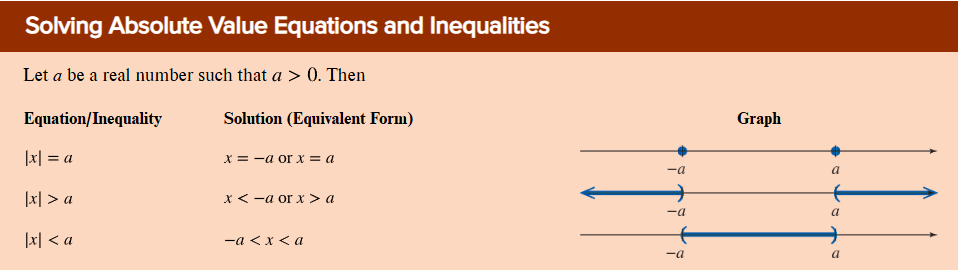
\includegraphics[width=1\linewidth]{스크린샷 2026-10-25 155758.png} 
\end{figure}
Solve the absolute value intequalities. 
\vspace{1.5em}

1. $|x|=5, |x|<5, |x|>5$

\vspace{4.5em}

2. $|x|=-5, |x|<-5, |x|>-5$

\vspace{4.5em}

3. $5\leq\vert 2x-1\vert$
\vspace{4.5em}

4. $12\leq \vert 9-4x\vert -2$

\vspace{4.5em}

5. $4>-1\left\vert \frac{2x+1}{4}  \right\vert$

\vspace{4.5em}

6. $8<\vert 4-3x\vert +12$
\vspace{3.5em}
\section{Absolute Value Inequalities, alternative method}

\begin{figure}[htbp]
    \centering
    % Replace "my_image" with your actual file name (without extension)
    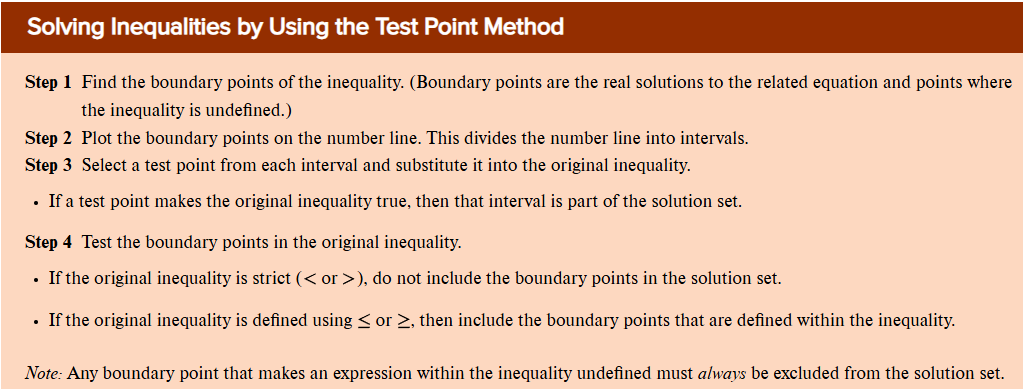
\includegraphics[width=1\linewidth]{스크린샷 2026-10-25 160523.png} 
\end{figure}
Solve the absolute value intequalities. 
\vspace{1.5em}

1. $x+6<-2$ and $5x<30$

\vspace{4.5em} 

2. $5x+2x\geq -21$ and $-9x+3x\geq -24$ 

\vspace{4.5em} 

3. $\frac{5}{2}(x+2)<-6 $ and $\frac{3}{4}(x-2)<1 $ 

\vspace{4.5em} 

4. $-8\geq -3x-2$ and $3(x-7)+16>4x$ 

\vspace{4.5em}


\end{document}